\section{Upsampling}
\begin{frame}{}
    \LARGE Image Segmentation: \textbf{In-Network Upsampling}
\end{frame}

\begin{frame}{In-Network Upsampling: Unpooling}
    \begin{figure}
        \centering
        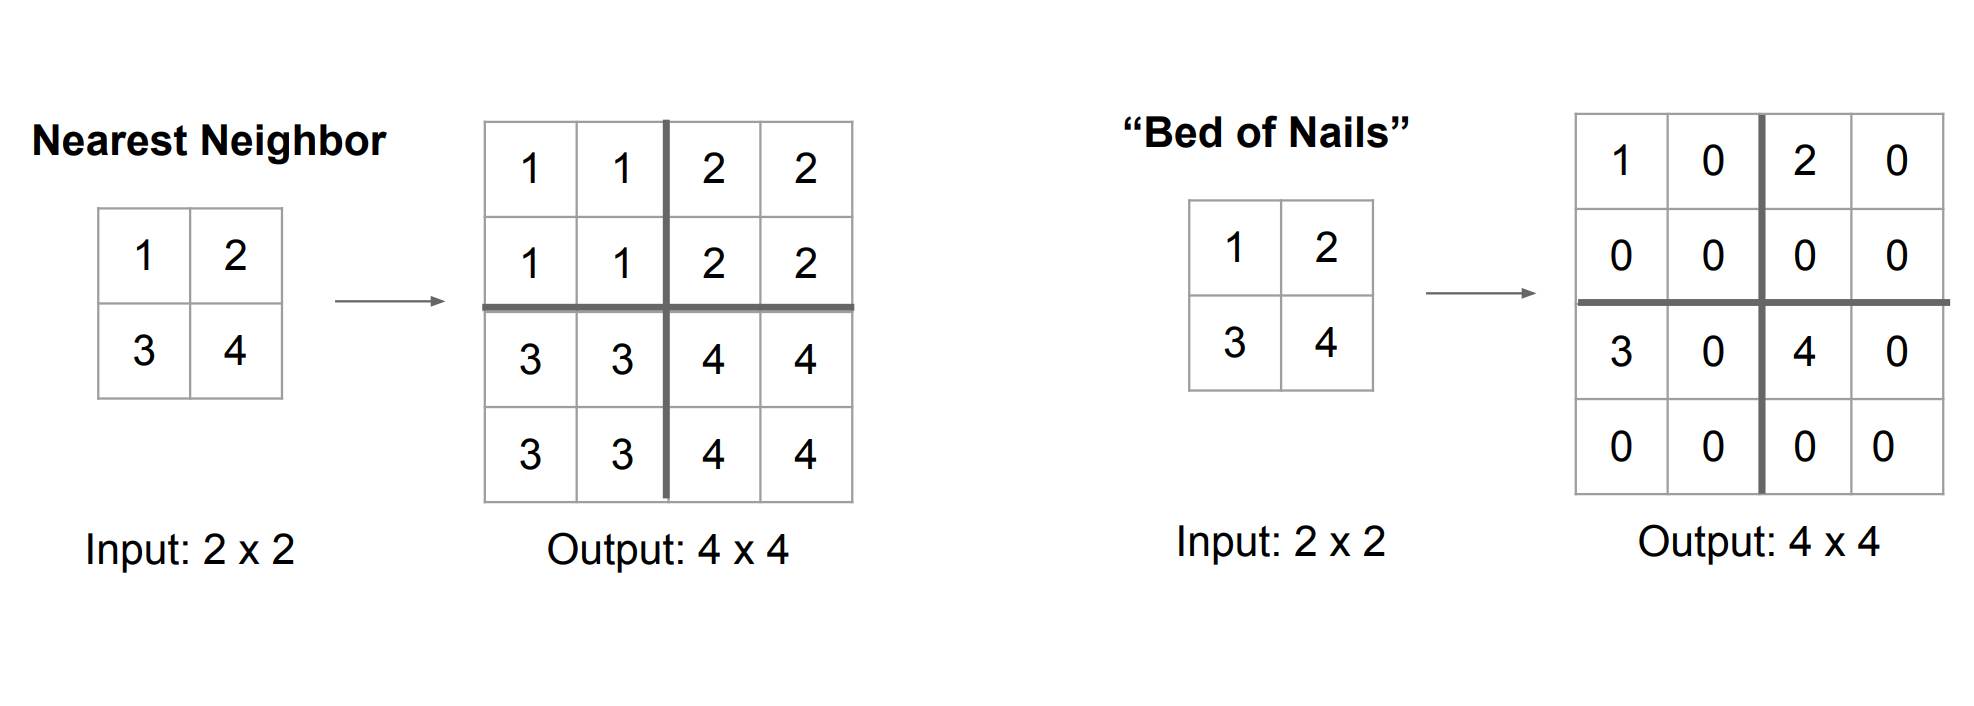
\includegraphics[width=1.0\textwidth,height=1.0\textheight,keepaspectratio]{images/segmentation/upsample_1.png}
    \end{figure}
\end{frame}

\begin{frame}{In-Network Upsampling: Max Unpooling}
    \begin{figure}
        \centering
        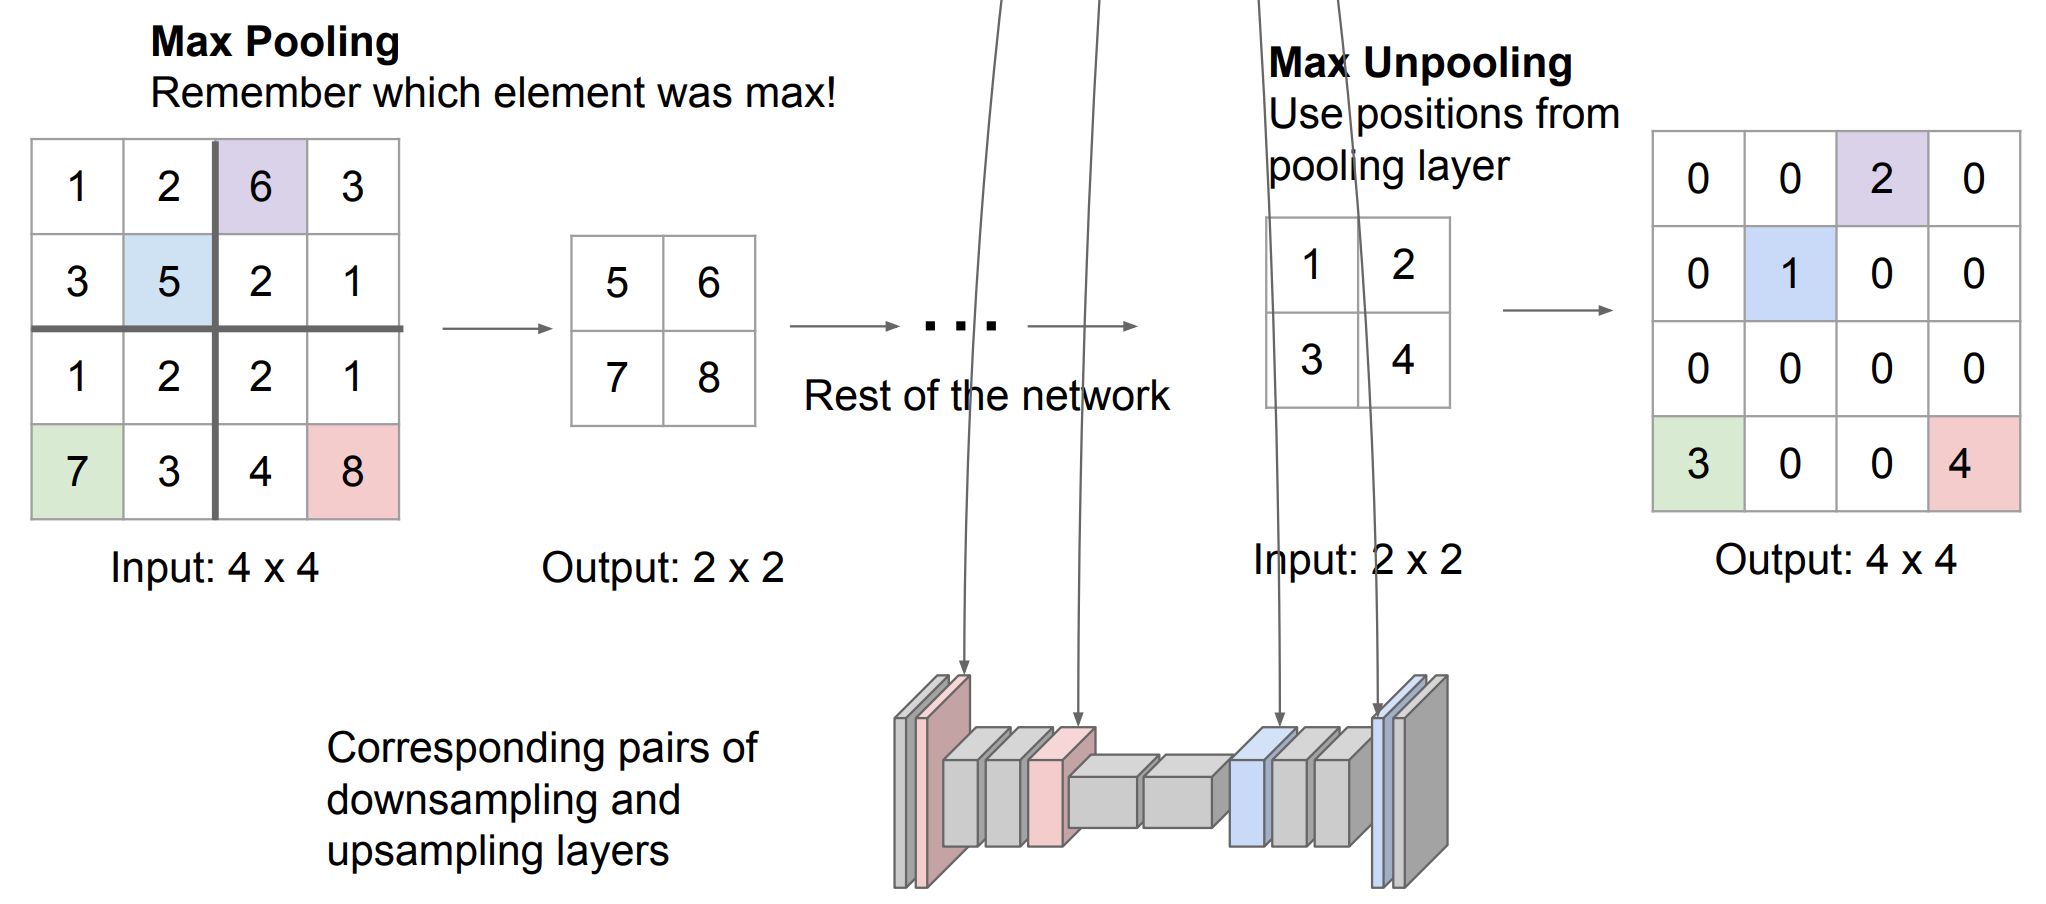
\includegraphics[width=1.0\textwidth,height=1.0\textheight,keepaspectratio]{images/segmentation/upsample_2.png}
    \end{figure}
\end{frame}

\begin{frame}[allowframebreaks]{Learnable Upsampling: Transposed Convolution}
\begin{figure}
\centering
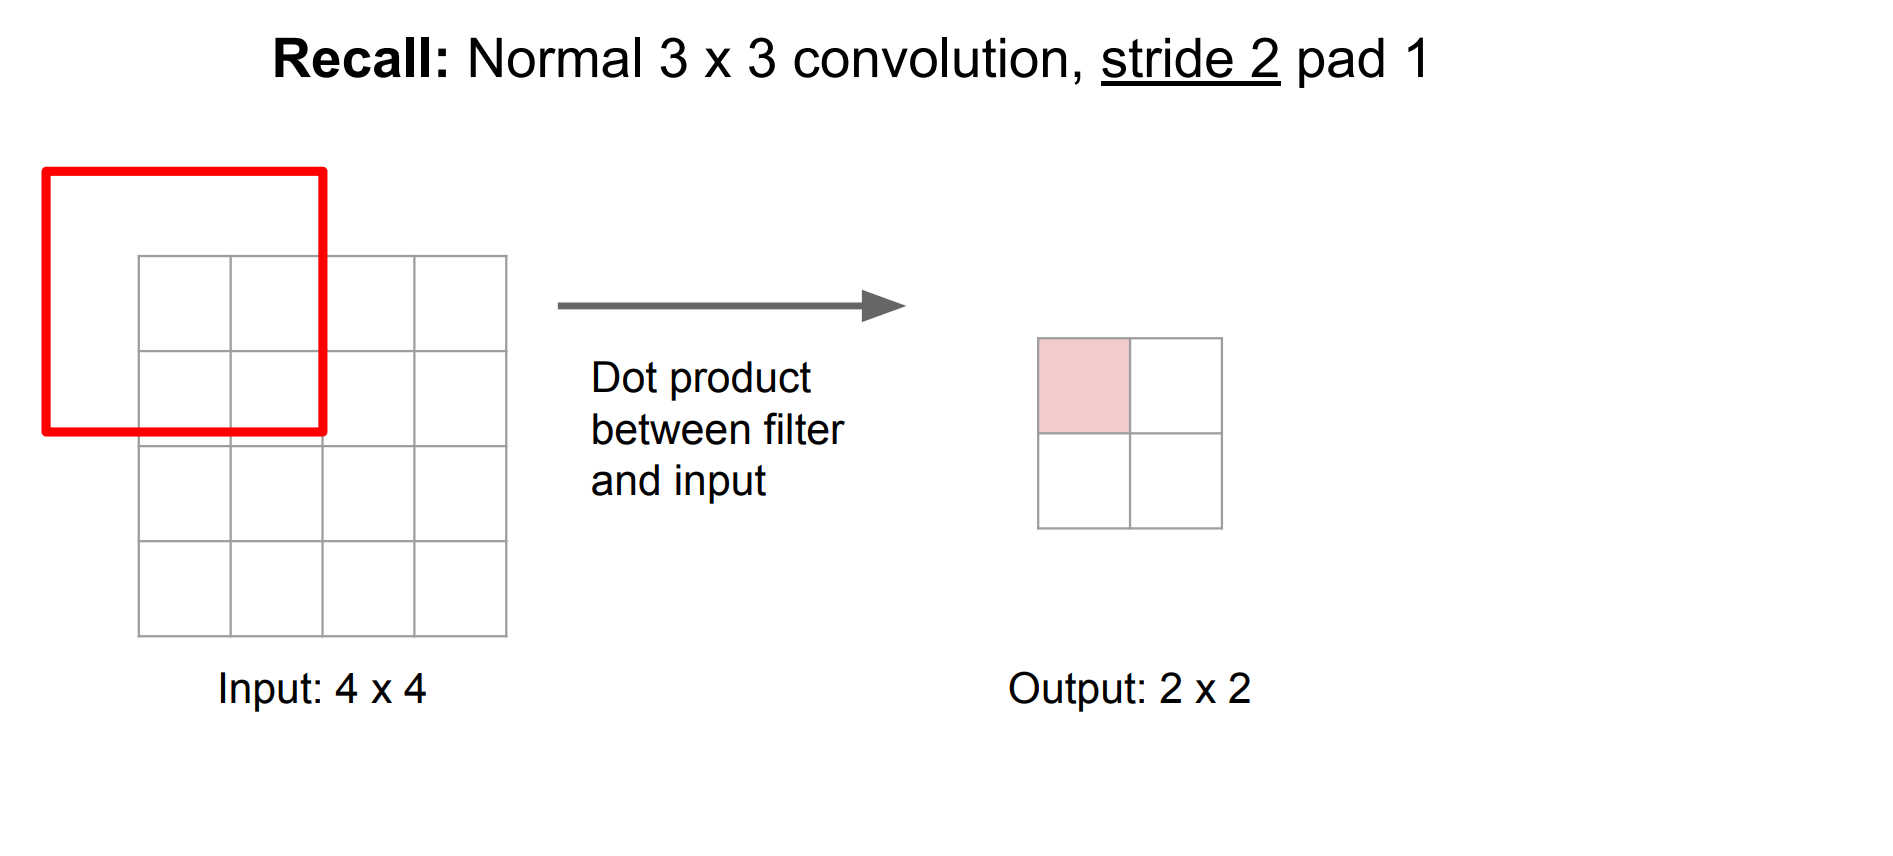
\includegraphics[width=1.0\textwidth,height=1.0\textheight,keepaspectratio]{images/segmentation/upsample_3.png}
\end{figure}

\framebreak

\begin{figure}
\centering
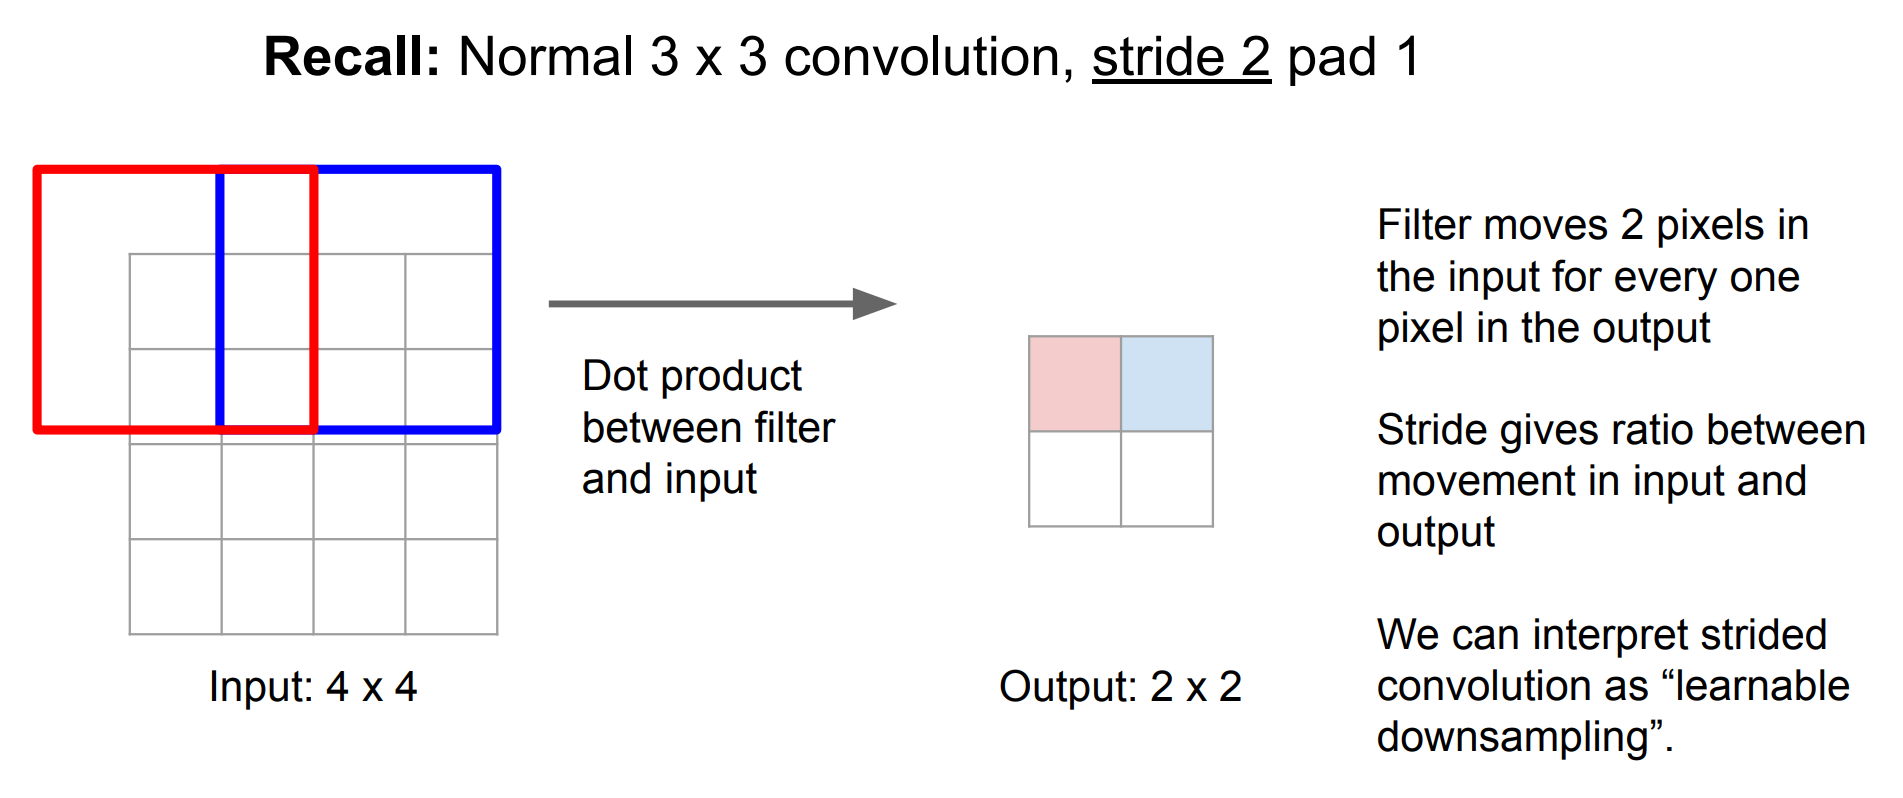
\includegraphics[width=1.0\textwidth,height=1.0\textheight,keepaspectratio]{images/segmentation/upsample_4.png}
\end{figure}

\framebreak

\begin{figure}
\centering
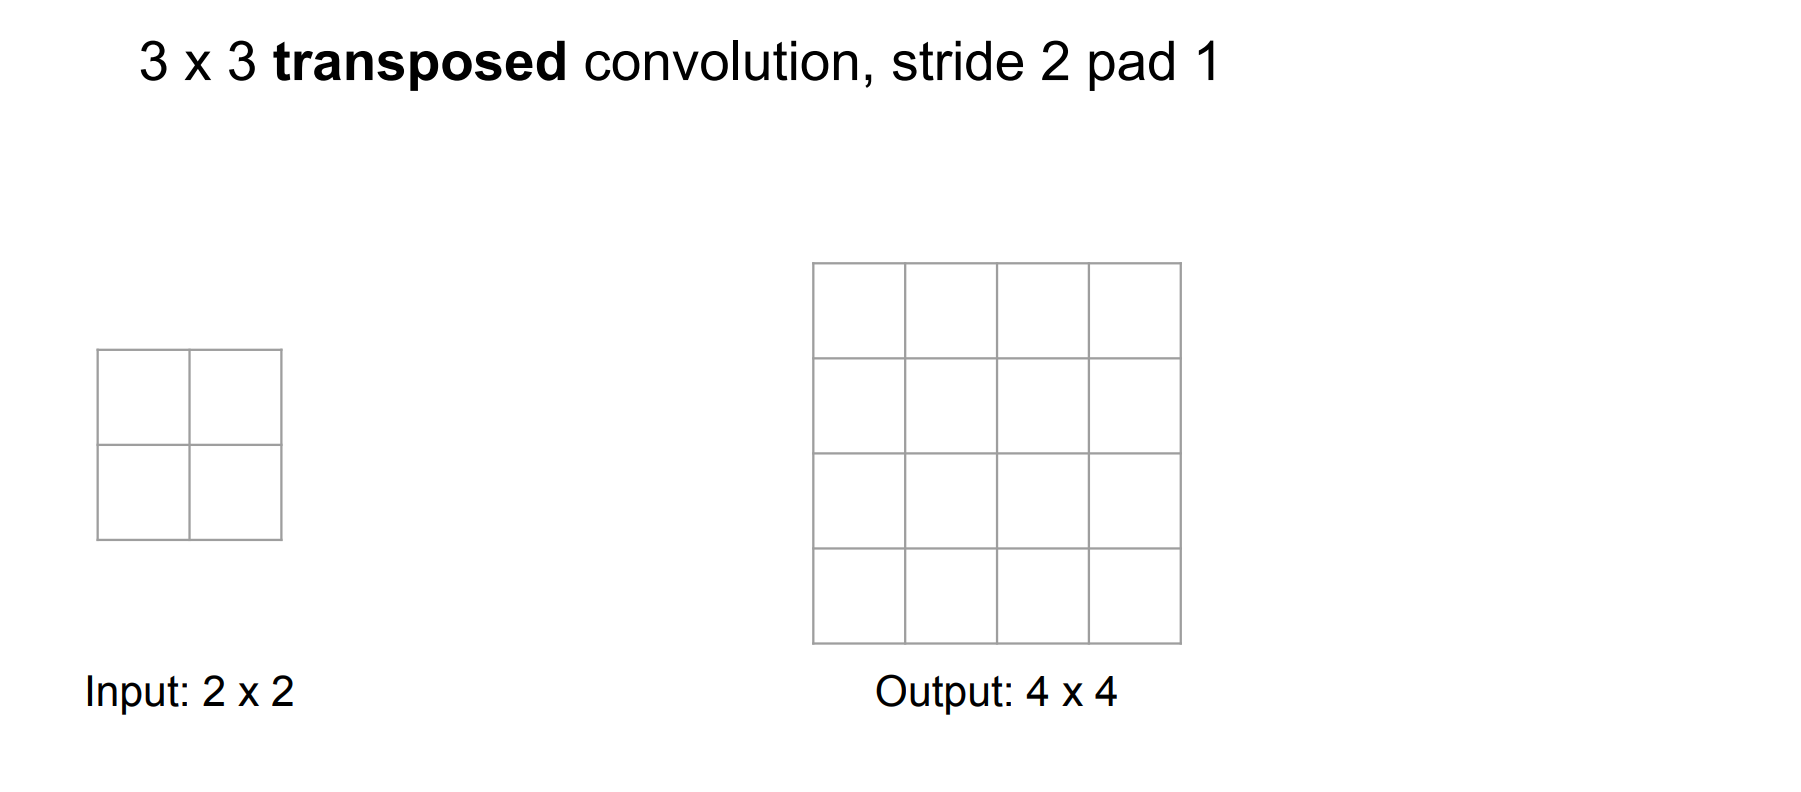
\includegraphics[width=1.0\textwidth,height=1.0\textheight,keepaspectratio]{images/segmentation/upsample_5.png}
\end{figure}

\framebreak

\begin{figure}
\centering
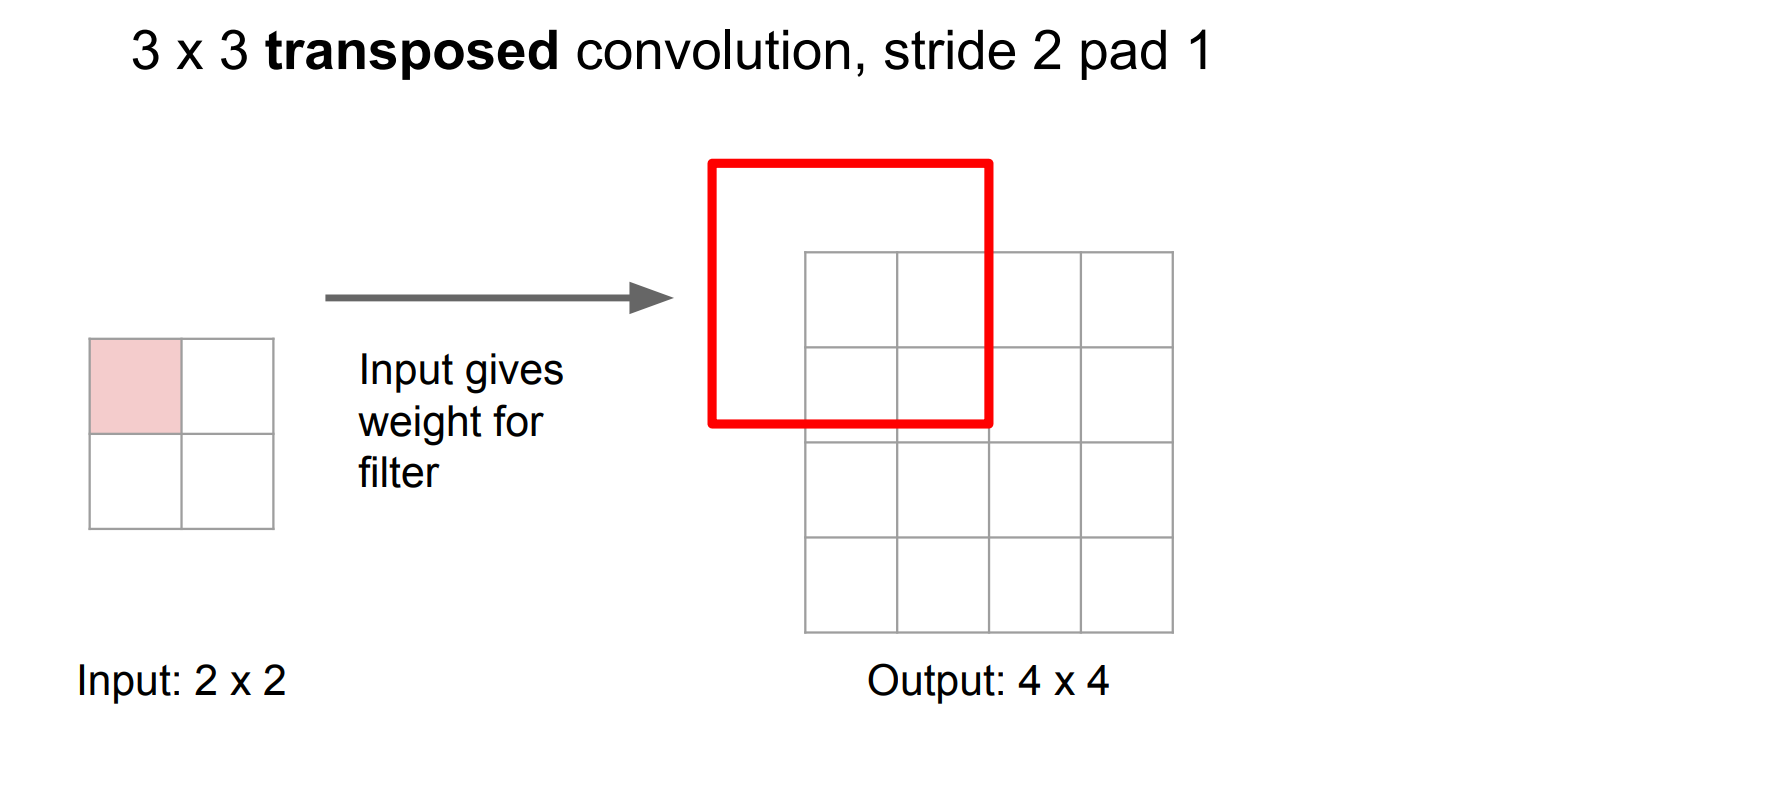
\includegraphics[width=1.0\textwidth,height=1.0\textheight,keepaspectratio]{images/segmentation/upsample_6.png}
\end{figure}

\framebreak

\begin{figure}
\centering
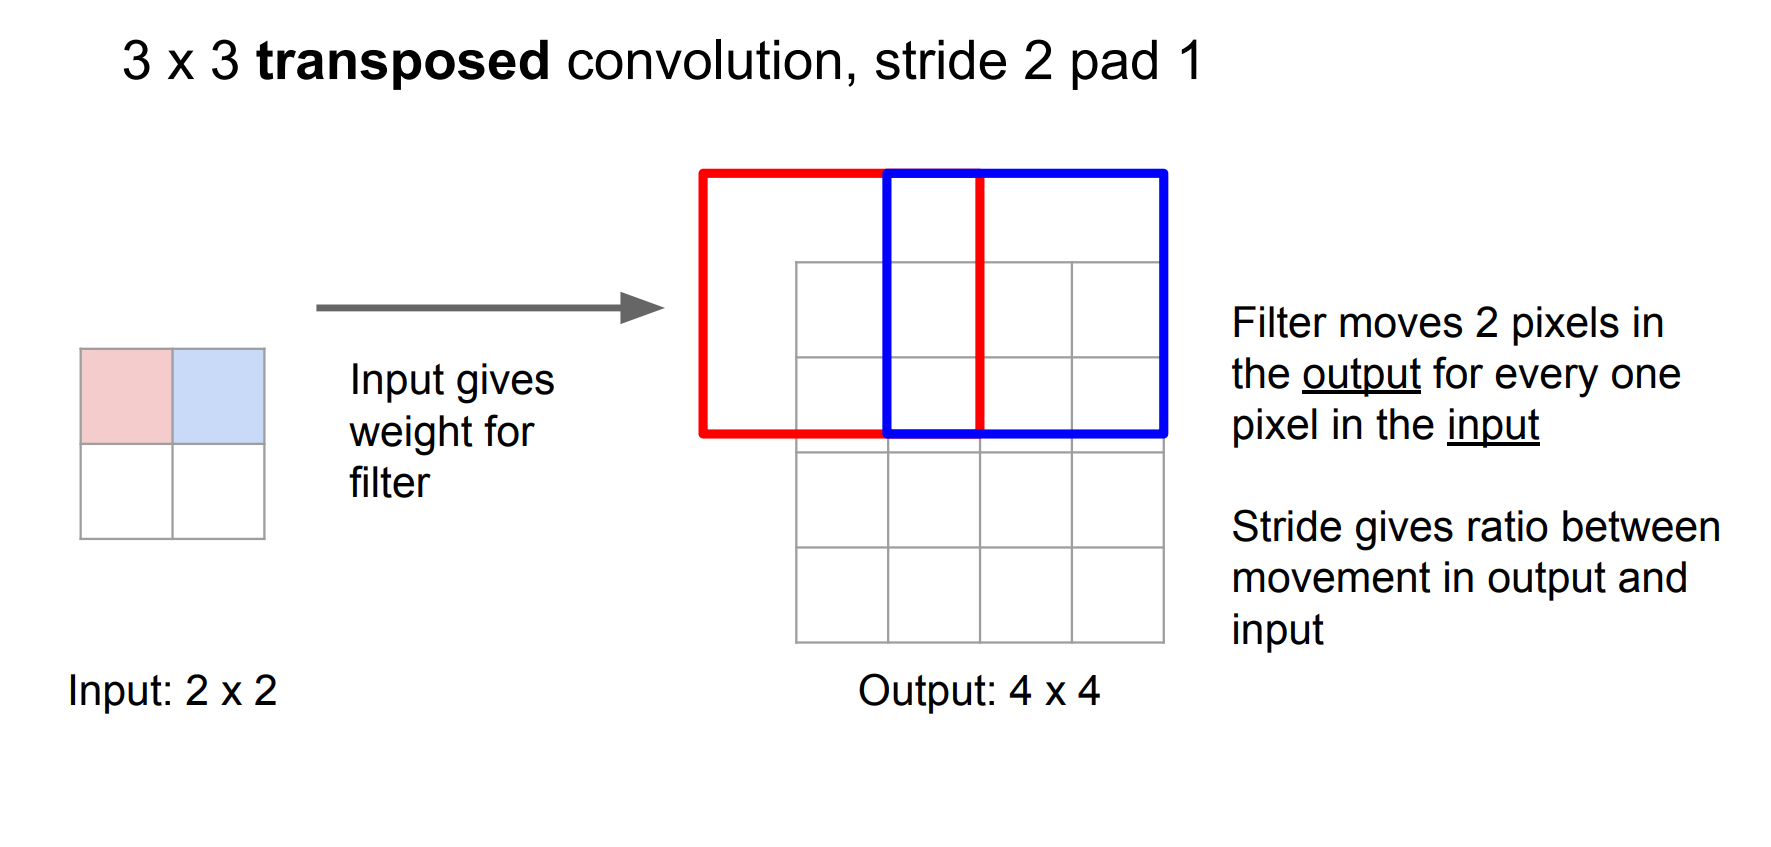
\includegraphics[width=1.0\textwidth,height=1.0\textheight,keepaspectratio]{images/segmentation/upsample_7.png}
\end{figure}

\framebreak

\begin{figure}
\centering
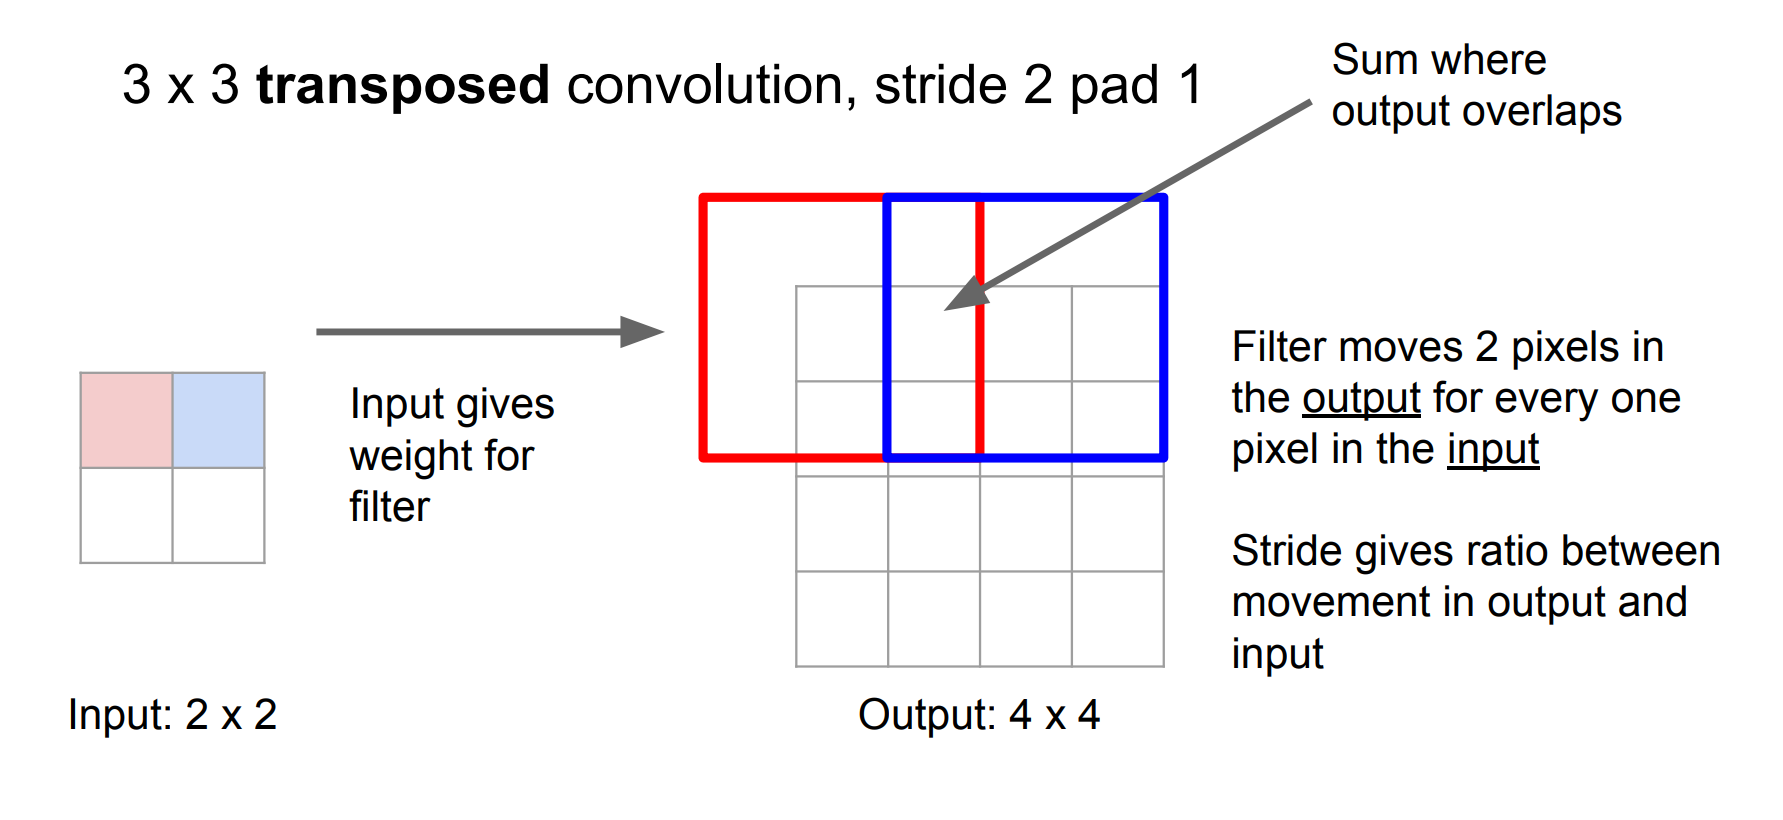
\includegraphics[width=1.0\textwidth,height=1.0\textheight,keepaspectratio]{images/segmentation/upsample_8.png}
\end{figure}

\end{frame}